\documentclass{article}
\usepackage{hyperref}
\usepackage{mathtools}
\usepackage{CJKutf8}
\usepackage{amssymb}
\usepackage{geometry}
\usepackage{enumerate}
\usepackage{multicol} 
\usepackage{graphicx} 

\geometry{a4paper} 

\begin{document}
\begin{CJK}{UTF8}{gkai}

\title{异面直线及其所成角}
\date{}
\author{张舒悦}
\maketitle

\section{教学目标}
\begin{enumerate}
\item 理解异面直线的概念.
\item 判定异面直线.
\item 确定异面直线所成角, 并计算其大小.
\end{enumerate}

\section{教学重点}
\begin{enumerate}
\item 判定异面直线.
\item 确定异面直线所成角.
\end{enumerate}

\section{教学难点}
\begin{enumerate}
\item 运用反证法证明异面直线.
\item 运用三角知识计算异面直线所成角.
\end{enumerate}

\section{教学过程}
%\begin{multicols}{2}
%1\columnbreak \\ 2
%\end{multicols}
%\textcircled{1}
\subsection{引入}
\subsubsection{异面直线}
在正方体$ABCD-A_1B_1C_1D_1$中, \\
\textcircled{1}直线$AB$与直线$A_1B_1$的位置关系? 平行. 无交点.\\
\textcircled{2}直线$AB$与直线$BD$的位置关系? 相交. 一个交点B.\\
\textcircled{3}直线$AB$与直线$B_1C_1$的位置关系?\\
*提问: 是否平行? 是否相交? 既不平行也不相交.\\
*提问: 3与12的不同之处? \\
根据公理2的推论2与3, 12两种情况中均存在一个平面经过这两条直线, 而3中, 这样的平面不存在. 这也就是说任何一个平面都不可能同时经过这两条直线. 我们不可能把这两条直线置于同一个平面内.\\
*板书:我们把不能置于同一平面的两条直线$l_1 l_2$叫做异面直线.\\
*提问: 交点数量? \\
*板书: \\
\begin{center}
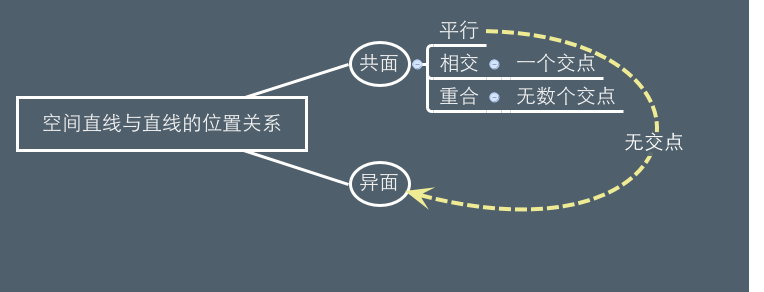
\includegraphics[scale=0.4]{/Users/shuyue/Documents/TeX/1.png}
\end{center}
在空间直线间的位置关系中, 无交点不一定平行.\\

\subsubsection{两条异面直线的直观图}
*板书: 随意作两条直线.\\
没有异面的视觉效果, 所以有必要借助辅助平面.\\
要点在于有异面的视觉效果, 既不相交也不平行.\\
这样作图就一定是异面直线吗?\\

\subsection{证明异面直线}
已知: 直线$l$与平面$\alpha$相交于点$A$, 直线$m$在平面$\alpha$上, 且不经过点$A$, 求证: 直线$l$与$m$是异面直线.\\
*作图: \\
*引导: 回顾所学公理定理及其推论, 是否有关于异面直线的?\\
*提问: 那有没有关于共面直线的?\\
公理3及推论123.\\
*提问: 共面直线与异面直线的关系是什么样的?\\
对立的关系, 不是共面则是异面, 二者仅可取其一并且必须取其一.\\
我们先假设共面, 回顾反证法证明步骤.\\
利用条件, 导出矛盾, 得出假设不成立. 这样只可能是异面直线.\\
证明: 假设直线$l$与直线$m$不是异面直线, 那么直线$l$与直线$m$是共面直线. 设直线$l$与直线$m$在平面$\beta$上.\\
*注意: 不能使用$\alpha$, 要与已知区别开.\\
$\because A \notin m$,\\
$A \in \alpha$, $m \subset \alpha$; $A \in \beta$, $m \subset \beta$.\\
$A$与$m$满足推论1的条件, \\
$\therefore$ 因而$A$与$m$确定一个平面. 这个平面现在既是$\alpha$, 又是$\beta$.\\
$\therefore \alpha = \beta$.\\
$\because l \subset \beta$.\\
$\therefore l \subset \alpha$.\\
与已知中$l \bigcap \alpha = A$矛盾, 假设不成立. 因而直线$l$与直线$m$是异面直线.\\
\newline
三种作图方式中12可以用这个真命题来判定; 3则可以用既不平行又不相交来判定.

\subsection{异面直线所成角}
我们如何定性地更精确地来描述异面直线的相对位置关系?\\
通过作平行线使两条直线交于一点, 并引入角的概念.\\
*提问: 回顾平面两直线夹角的定义.
\subsubsection{定义}
对于异面直线$a$和$b$, 在空间任取一点$P$, 过$P$分别作a和b的平行线$a'$和$b'$, 我们把$a'$和$b'$所成的*锐角或直角*叫做异面直线$a$与$b$所成的角.\\
*作图:\\
*提问: 这个角的大小与P点选取是否有关?\\
由定理1保证, 与P点选取无关. 也就是说, 所成角不是唯一的, 但是角的大小是唯一的.\\
这个点可以在空间中的任何位置, 包括可以在直线$a$或者$b$上.\\
若点选取在其中一条直线上, 只需要作一条平行线.\\
根据图形特征来选取点P.\\
\newline
*提问: 异面直线所成角的范围?\\
直角则两直线异面垂直, 记作$l_1\perp l_2$; 零角是共面情形, 两直线平行或者重合. \\
$(0, \frac{\pi}{2}]$.

\subsubsection{例题}
正方体$ABCD-A_1B_1C_1D_1$的棱长为$a$, 求下列异面直线所成的角的大小:\\
\textcircled{1}$AB$与$B_1C_1$;\\
$\because BC \parallel B_1C_1$.\\
$\therefore \angle ABC$ 即为所成角或其补角, 大小为$90^ \circ$.\\
\textcircled{2}$A_1B$与$CC_1$;\\
$\because BB_1 \parallel CC_1$.\\
$\therefore \angle A_1BB_1$ 即为所成角或其补角, 大小为$45^ \circ$.\\
\textcircled{3}$AB_1$与$BC_1$.\\
$\because AD_1 \parallel BC_1$.\\
$\therefore \angle B_1AD_1$ 即为所成角或其补角.\\
*引导: 问题转化为求该角的大小.
$\because B_1A = D_1A = B_1D_1 = \sqrt{2}a$.\\
$\therefore \vartriangle B_1AD_1$为等边三角形, $\angle B_1AD_1 = 60^ \circ$.\\
$\therefore$ 所成角大小为$60^ \circ$.\\
\newline
*板书: 求异面直线所成角大小的步骤:\\
\begin{itemize}
\item 选取合适的角.
\item 利用余弦定理, 勾股定理逆定理, 反三角函数等知识求角的大小.
\item 确认是锐角或者直角.
\end{itemize}

\subsection{小结}
\begin{itemize}
\item 异面直线的一般证明方法: 反证法.
\item 异面直线所成角与点的选取无关.
\end{itemize}

\subsection{思考题}
长方体$ABCD-A_1B_1C_1D_1$中, $AB = a$, $AA_1 = b$, $AD = c$. 求下列异面直线所成的角的大小:\\
\textcircled{1}$AB$与$B_1C_1$;\\
\textcircled{2}$A_1B$与$CC_1$;\\
\textcircled{3}$AB_1$与$BC_1$.\\


\end{CJK}
\end{document}